\chapter{Appendix B: Stable computation of likelihood values}
\label{AppendixB}

The stable computation of likelihood values is an essential component of running algorithms which resolve the posterior distribution. This can be an issue as the value of the likelihood for a given set of parameters can be extraordinarily small, to the point where these values approach or cross the limits of what can be stored in a computers memory. \\

Consider a unit hyper sphere that is located in a unit hyper cube. In low dimensions the sphere inside a cube takes up a large \% of the cubes volume. However, as the dimension increases this volume very rapidly diminishes. Figure \ref{hyper-objects} illustrates this relationship. The purpose of this example is to demonstrate that high dimensional spaces are very sparse. Geophysical inverse problems suffer particulary from this dimensionality, our images have many unknown parameters. Hence problems arising as a result of dimensionality, often reffered to as \textit{the curse of dimensionality}, are of particular importance to geophysics. \\

\begin{figure}[H]
	\centering
	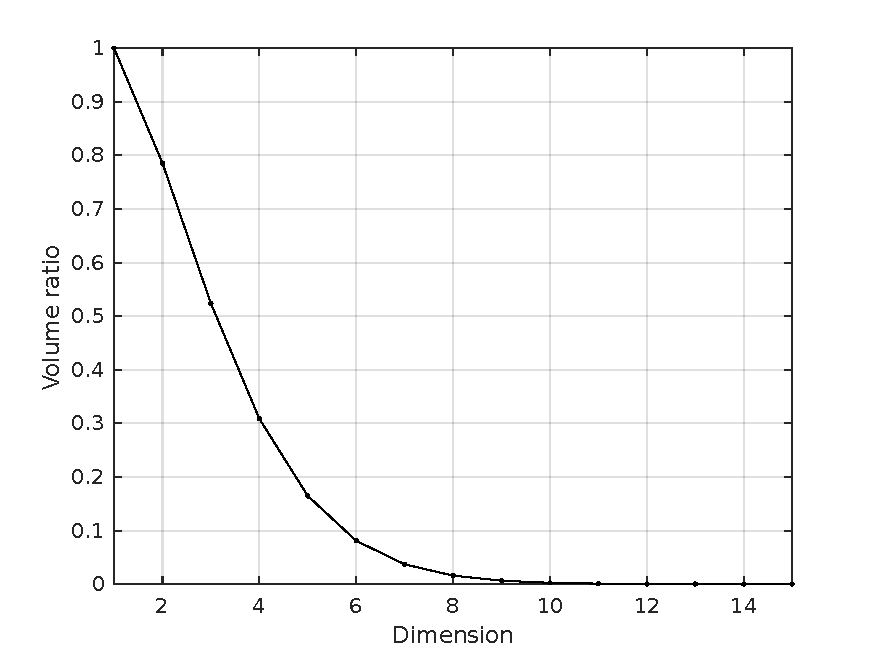
\includegraphics[scale=0.7]{hyper-objects.pdf}
	\caption{The volume ratio of a unit hyper sphere, $2\pi^{d/2}r^d/d/\Gamma(d/2)$, inside a unit hyper cube, $(2r)^d$, as a function of dimension, $d$. This example is inspired by Marko Laine.}
	\label{hyper-objects}
\end{figure}

For a likelihood distribution over a sparse high dimensional space, the majority of the space will be extraordinarily empty - i.e. with very low probability. Considering probability is a value between 1 and 0, that means a lot of parameter space will have a liklihood very close to 0. Given this circumstance it is essential to be able to accurately compute and compare extremely small probability values. The risk of improper evaluation and comparison is erraneious steps in algorithms and a divergence from the posterior the algorithm is supposed to be sampling. In short your solution will be wrong. \\

How to overcome this issue? The solution is to compute the natural logarithm of the likelihood. Figure \ref{nat-log} shows taking the natural logarithm of probability values. The result is very small probability values become very large negative numbers.

\begin{figure}[H]
	\centering
	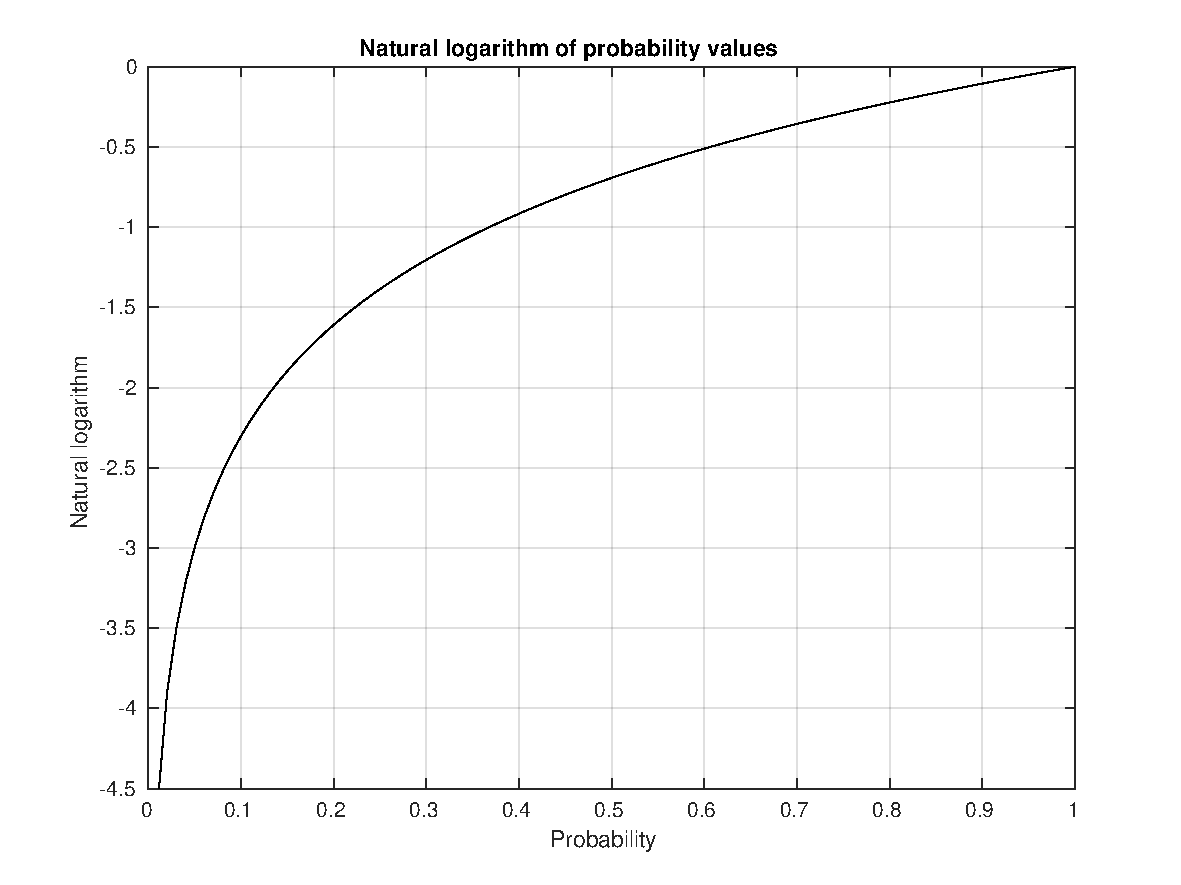
\includegraphics[scale=0.7]{nat-log.pdf}
	\caption{The natural logarithm of probability values}
	\label{nat-log}
\end{figure}

These very large negative numbers transform a very small value, close to or crossing the limits of CPU memory, into a large number which can be easily stored. \\

For a Gaussian likelihood, taking the natural logarithm of an unnormalizaed likelihood is in effect removing the exponentional term. Consider the likelihood as in equation \ref{likelihood-2}. Repeated here
\begin{equation}
\mathcal{L}(\bm{\theta}|\bm{y}) \propto \text{exp}\bigg[-\frac{1}{2}(\bm{y}-\bm{g}(\bm{\theta}))^T(C_{\mathcal{M}}+C_{\mathcal{D}})^{-1}(\bm{y}-\bm{g}(\bm{\theta}))\bigg]
\label{repeat-likelihood-2}
\end{equation}
For $l(\bm{\theta}|\bm{y}) = \text{ln}(\mathcal{L}(\bm{\theta}|\bm{y}))$
\begin{equation}
l(\bm{\theta}|\bm{y}) \propto -\frac{1}{2}(\bm{y}-\bm{g}(\bm{\theta}))^T(C_{\mathcal{M}}+C_{\mathcal{D}})^{-1}(\bm{y}-\bm{g}(\bm{\theta}))
\label{log-likelihood}
\end{equation}
Reference to the negative log-likelihood would then mean
\begin{equation}
-l(\bm{\theta}|\bm{y}) \propto \frac{1}{2}(\bm{y}-\bm{g}(\bm{\theta}))^T(C_{\mathcal{M}}+C_{\mathcal{D}})^{-1}(\bm{y}-\bm{g}(\bm{\theta}))
\label{negative-log-likelihood}
\end{equation}
The negative log-likelihood is then a large positive number for very small probability values. Often minimization of an equation in the form of equation \ref{negative-log-likelihood} is the goal of linearized inversion schemes. Herein lies a connection between the likelihood function and linearized schemes, the result of a successful lineared inversion represents the minimum of the negative log-likelihood, $-l(\bm{\theta}|\bm{y})$. Which is also the maximum likelihood value. However our goal is generally broader. To explore the joint posterior distribution, a function of both likelihood and prior. This goal in high dimensional space neccessitates Markov chain Monte Carlo (MCMC) sampling. So how does our shift to working with the natural logarithm of the likelihood impact this algorithm? \\

For a MCMC algorithm with stationary distribution which is the posterior $p(\bm{\theta}|\bm{y})$, the key ingredient is evaluating the Metropolis-Hastings acceptance ratio, $\alpha$
\begin{equation}
\alpha = \frac{\mathcal{L}(\bm{\theta^*}|\bm{y})\ p(\bm{\theta^*})}{\mathcal{L}(\bm{\theta}|\bm{y})\ p(\bm{\theta})}
\label{acceptance-ratio}
\end{equation}
Where $^*$ represents a candidate move from the proposal distribution $q(\bm{\theta},.)$. As long as the proposal distribution is a symmetric distribution the ratio $q(\bm{\theta^*},\bm{\theta})/q(\bm{\theta},\bm{\theta^*})$ does not need to be computed as part of $\alpha$.\\

Hence, the ratio of posterior values needs to be computed at each time step over the parameter space. The raw posterior values will be prone to numerical underflow due to the limits of CPU memory, hence the log values for the likelihood must be used in this calculation. How does the form of $\alpha$ get adjusted within a computer program to ensure stable and reliable computation?\\

This shift represents a major divergence between how the theory is established in equation form, and the practical application in computer code. It also eventually leads to a major issue for joint inversion schemes. \\

Consider we have access to the log-likelihood and log-prior. Recall the logarithm rules where $\text{ln}(xy) = \text{ln}(x)+\text{ln}(y)$ and $\text{ln}(x/y) = \text{ln}(x)-\text{ln}(y)$. Then
\begin{equation}
\alpha = \text{exp}\Big[\Big(l(\bm{\theta^*}|\bm{y})\ -\ l(\bm{\theta}|\bm{y})\Big)\ +\ \Big(\text{ln}\big(p(\bm{\theta^*})\big)\ -\ \text{ln}\big(p(\bm{\theta})\big)\Big)\Big]
\end{equation}
The resulting acceptance-ratio computed here will be equivilent to equation \ref{acceptance-ratio}, however, now the probability densities recquired in the computation will be restricted to large numbers, stable in their computation and comparison. The end result, a reliable MCMC algorithm.\\

% Introfuce issue which arises due to the different scale of the terms in this new Metropolis-Hastings acceptance ratio

